\documentclass[letterpaper,12pt]{article}
\setlength{\headheight}{14.49998pt}
\usepackage{fancyhdr}
\usepackage{lipsum,graphicx}
\usepackage{bookmark}
\usepackage{amsmath, amsfonts, amssymb, ragged2e}
\usepackage{listings}
\graphicspath{ {./images/} }
\title{Summary of CPEN 221}
\author{Tom Wang}
\date{Fall, 2023}

\fancypagestyle{plain}{
    \fancyhf{}
    \fancyhead[L]{Tom Wang}
    \fancyhead[R]{\thepage}
}

\begin{document}

\maketitle
\thispagestyle{plain}

\section{Intro}

Topics going to be covered in CPEN 221:
\begin{itemize}
    \item Specifications
    \item typing and simple static analysis
    \item testing
    \item abstraction (procedural abstraction and data abstraction)
    \item abstract data types
    \item type hierarchies
    \item concurrency
\end{itemize}

\section{Types}

A type is a set of values and the operations that are permitted on the values.

\subsection*{OOP}
In OOP, reference types are objects and primitive types
are not. The name of the object is the reference to the object.

The object will have a constructor so that we can construct/create the object.
\subsection*{User-defined types}
The intention of a type is that all interaction with values of that type be
through the operations defined for that type.

Defensive programming:

Build a wall to limit the access from others. E.g., private.

\subsection*{Type safety}

Type safety refers to a programming language's support for detecting type
errors.

\begin{itemize}
    \item Static analysis: Analysis performed during the compilation stage (or before a
          program is executed)
    \item Dynamic analysis: Runtime analysis
\end{itemize}
Languages that can support stronger static analyses typically lead to stronger correctness guarantees.

\section{Exception}
\subsection*{Definations}
Exceptions are contracts that are supported by multiple programming languages.
Exception mechanisms allow programmers to indicate problems and mechanisms
include techniques for method clients to recover from problematic situations in
a reasonable manner.

Java provides \textbf{throw} mechanism to indicate a problem or special
situation. \textbf{catch} mechanisms can handle an exception thrown by the
method used.
\subsection*{Type of exception}
Java provides two exception types: \textbf{checked and unchecked}.
\begin{itemize}
    \item Checked exception means it is checked by the compiler. It must be handled or
          declared the exception itself.
    \item Unchecked exceptions are used to signal bugs. These exceptions are not expected
          to be handled.
    \item All exceptions may have a message associated with them. If not provided in the
          constructor, the reference to the message string is null.
\end{itemize}
\subsection*{Throwable hierachy}
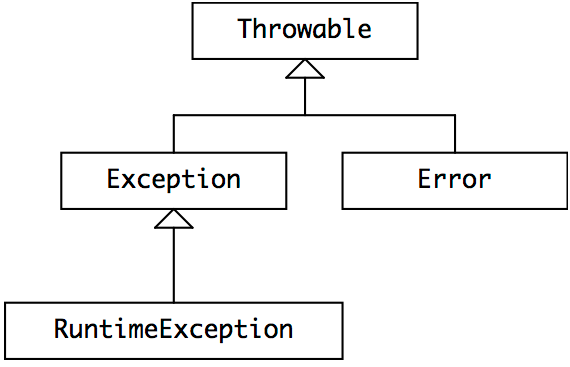
\includegraphics{./summary_image/Throw_Hierarchy.png}

Throwable is the class of objects that can be thrown or caught. Any object used
in a throw or catch statement, or declared in the throws clause of a method,
must be a subclass of Throwable.

Error is a subclass of Throwable that is reserved for errors produced by the
Java runtime system, such as StackOverflow­Error and OutOfMemory­Error. For
some reason, Assertion­Error also extends Error, even though it indicates a bug
in user code, not in the runtime. Errors should be considered unrecoverable,
and are generally not caught.

\begin{itemize}
    \item RuntimeException, Error, and their subclasses are unchecked exceptions. The
          compiler doesn't require these to be declared in the throws clause of a method
          that throws them and doesn't require these to be caught or declared by a
          caller of such a method.
    \item All other throwables — Throwable, Exception, and all of their subclasses except
          for those of the RuntimeException and Error lineage — are checked exceptions.
          The compiler requires these exceptions to be caught or declared when they can be thrown.
\end{itemize}
When you define your own exceptions, you should either subclass RuntimeException (to make it an unchecked exception) or Exception (to make it checked).
\subsection*{Exception design considerations}
\begin{itemize}
    \item If you design a method to have its own (new) exception, you have to create a
          new class for the exception.
    \item If you call a method that can throw a checked exception, you have to wrap it in
          a try-catch statement (even if you know the exception will never be thrown).
\end{itemize}
\textbf{Refined rule: }
You should use an unchecked exception only to signal an unexpected failure (typically, a bug), otherwise, you should use a checked exception.

\section{Computing system}
\subsection*{fetch-and-execute cycle}
CPU fetches instruction from memory and then executes it. 

Registers keep the values inside the CPU, program counter keeps track of the instruction address.

\subsection*{Asynchronous Events}
CPU checks data over and over again and executes when the desired data arrives. It is called polling. However, it wastes performance to keep waiting. 

Instead, the CPU gets interrupts, which stalls the current task and handles interrupts. 

Processes are individual tasks that the CPU is working on. Note that processes can have multiple streams of execution called threads. 

\subsection*{Java Virtual Machine}
Low\-level language can be translated directly to assembly and then machine language by the compilers. However high\-level languages like Java need an intermediate step. 

JVM is an interpreter that translates instructions one by one. Compilers translate Java to Java Bytecode program, which is a machine language for JVM. Then Java interpreter translates Java Bytecode to the local machine language. So it can be used across platforms. 

To solve the problem that it takes time to translate between JVM and local machine, Java introduced just\-in\-time compilers which translates from JVM to machine code while compiling to reduce time. 
\section{Program}

\subsection*{Computation and Memory}

In the old days, the compiler explicitly decides the address of data. However, the challenge is that no other program can use it anymore.

The modern approach is to indicate an offset of the base address. It allows multiple programs to run at the same time. Also, it allows the same data to be accessed by different programs giving different offsets.

Compilers use offset from a stack pointer to track address. Stack is \textbf{Last-in-first-out}. So the last function called will be the first function executed.

Memory is therefore divided into a few regions, one of which is called the stack and this is where local variables declared in a function are stored. Another region of memory that is useful is called the heap, and data whose sizes cannot be known ahead of time (at compile time) are stored on the heap.

CPU contains \textbf{Program Counter} (PC) to keep track of the memory address
of the instruction being executed. Normally, pc is incremented by 1 unless
conditional statements and function calls are given.

\subsection*{Call Stacks and Stack Frames}

When a function is called, a \textbf{stack frame} is created to support the function's execution. The stack frame contains the function's local variables and the arguments passed to the function by its caller. The frame also contains housekeeping information that allows the called function (the callee) to return to the caller safely.

\includegraphics*[scale = 0.3]{./summary_image/Stack_frame.png}

The stack pointer, \textbf{esp}, always points to the last item pushed in, which is the top of the stack. It specifically points to the first byte occupied by \textit{local buffer}, which is the lowest memory address in a stack containing live data.

Base pointer or frame pointer, \textbf{ebp}, points to a fixed location within the stack frame of the function currently running and provides a stable reference point for \textbf{accessing arguments and local variables}. (Using offset) Unlike esp, ebp is mostly maintained by program code with little CPU interference.

Finally, the \textbf{eax} register is used by convention to transfer return values back to the call for most C data types.

Check out CN5.3. For more details.

Summarize the steps:
\begin{enumerate}
    \item ``call main'':push return address onto the stack, jump into main
    \item ``push ebp'':save current ebp register values
    \item ``mov esp, ebp'':copy esp to ebp

          These are function prologue. The current value of ebp is saved to the top of
          the stack. esp is copied to ebp to establish a new frame.

          After some function calls it will call back to the original position.
\end{enumerate}

\section{Code testing and review}

\subsection*{Software Validation}
The purpose of validation is to uncover problems in a program and thereby
increase one's confidence in the program's correctness.

Validation includes:
\begin{itemize}
    \item Formal reasoning: usually called verification. Not so possible for large
          programs.
    \item Testing: Running the program on carefully selected inputs and checking the
          results.
    \item Code review: Having someone else carefully read your code and reason informally
          about it.
\end{itemize}

As a tester, you want to make the program fail.

We should test early and often. You write tests before you even write any code.
The development of a single function proceeds in this order:
\begin{enumerate}
    \item Specification for the function
    \item Tests that exercise the function
    \item Actual code. Once you pass the tests, you are done.
\end{enumerate}

\subsection*{Why software testing is hard}
Here are some approaches that do not work well:
\begin{itemize}
    \item Exhaustive testing: Space of possibility is too large to cover.
    \item Haphazard testing: (Just try it and see if it works) does not do anything. It
          will not increase confidence in the program.
    \item Random or statistical testing: Randomly testing a small portion of the software is
          not working. Software behaves discontinuously and discretely across the space
          of possible input.
\end{itemize}

\subsection*{Partitioning}
Test suite: a set of test cases that cover different aspects of a program's
behaviour.

We divide the input space into \textbf{subdomains}, each consisting of a set of
inputs. Taken together the subdomains completely cover the input space and
every input lies in at least one subdomain. Then we choose one test case from
each subdomain, and that is our test suite.

\includegraphics*{./summary_image/Partitioning example.png}

Bugs often occur at the boundary between subdomains. There are a few reasons:
\begin{itemize}
    \item Programmers often make off-by-one mistakes. For example, mess up $>$ and $\ge$.
    \item Some boundaries may need to be handled as special cases in the code.
    \item Boundaries may be places of discontinuity in the code's behavior. For
          example, \textbf{int} variable grows beyond its maximum positive value.
\end{itemize}

\subsection*{Two Extremes for Testing}
After partitioning the input space, we can choose how exhaustive we want the
test suite to be:
\begin{itemize}
    \item Full Cartesian product: Every legal combination of the partition dimensions is
          covered by one test case.
    \item Cover each part: Every part of each dimension is covered by at least one test
          case, but not necessarily every combination.
\end{itemize}

\subsection*{Blackbox and Whitebox Testing}

Specification is the description of the function's behaviour --- The types of
parameters, type of return value, and constraints and relationships between
them.

\textbf{Blackbox testing} means choosing test cases only from the specification, not the implementation of the function.

\textbf{Whitebox testing} means choosing test cases with knowledge of how the function is implemented.
You must take care that your test cases don't require specific implementation behaviour that isn't specifically called for by the spec.

\subsection*{Coverage}

\begin{itemize}
    \item Statement coverage: is every statement run by some test case?
    \item Branch coverage: For every if or while statement, are both the true or false
          directions taken by some test case?
    \item Path coverage: is every possible combination of branches --- every path through
          the program --- taken by some test case?
\end{itemize}

It is crucial to rerun your tests when you modify your code. It prevents the program
from regressing --- introducing other bugs. Running all your tests after every
change is called regression testing.

\subsection*{Coding style recommendations}

There are only two constants that many computer engineers and computer
scientists recognize as valid in and of themselves: 0, 1, and maybe 2. (Okay,
three constants.)

Other constant numbers need to be explained. One way to explain them is with a
comment, but a far better way is to declare the number as a constant with a
good, explanatory name.

Do not reuse parameters and variables. One purpose for each variable.

Add ``final'' to parameters or variables so that it will never be reassigned.

Use good names so that it is self-descriptive.

Three Cs:
\begin{itemize}
    \item Correct: find bugs
    \item Comprehensible: understandable
    \item Changeable: Readiness for change was considered by writing tests that only
          depend on behavior in the spec.
\end{itemize}

\section{Specifications}
A specification is a description of what an artifact does.

The contract between the producer and the consumer can be described using
preconditions and postconditions.

If the consumer promises to use the artifact in a particular fashion (this is
the precondition) then the producer guarantees that the artifact will behave in
the intended manner (which is the postcondition)

Precondition: The requirements on the input values.

Postcondition: The description of the output values.

Frame condition: Explain which element might change during the execution, avoid
unintended behavior.
\subsection*{The role of a spec}
With a spec:
\begin{itemize}
    \item the client (the user of a method or a class) agrees to rely only on information
          in the description/specification of the method or class for their part, and
    \item the implementer promises to support everything in the specification, and
          outside of the specification has perfect liberty to make implementation
          decisions.
\end{itemize}

A specification of a method can be concerned with the parameters and return
value of the method, but it should never discuss the local variables of the method
or private fields of the method's class.

\subsection*{Designing specifications}
\begin{itemize}
    \item Deterministic: Does the spec define only a single possible output for a given
          input or allow the implementor to choose from a set of legal outputs?
          \begin{itemize}
              \item Deterministic: when presented with a state satisfying the precondition, the
                    the outcome is determined.
              \item Non-Deterministic code is code that you expect to sometimes behave one way and
                    sometimes another.
          \end{itemize}
    \item Declarative: Does the spec just characterize what the output should be or does
          it explicitly says how to compute the output.
          \begin{itemize}
              \item Operational specs give a series of steps that the method performs; pseudocode
                    descriptions are Operational
              \item Declarative specs just give properties of the final outcome and how it is
                    related to the initial state.
          \end{itemize}
    \item Strong: Does the spec have a small set of legal implementations or a large set?
\end{itemize}

A specification A is stronger than or equal to a specification B if:
\begin{itemize}
    \item A's precondition is weaker than or equal to B's. (More or equal amount of
          allowed input)
    \item A's postcondition is stronger than or equal to B's, for the states that satisfy
          B's precondition. (Know more about the return value and outcome)
\end{itemize}

\section{Debugging}

The best defense against bugs is to make them impossible by design.

Static checking: catch them at compile time.

Dynamic checking: The system throws errors automatically. E.g. IndexOutOfBound
exception.

Make sure you know the difference between variables and pointers. Making
pointers final only keeps the address unchanged but not the thing it points to.

Fail fast to localize bugs. Use ``assert\(variable\)'' to check for errors.
Following are a few things you should assert:
\begin{itemize}
    \item method argument requirements
    \item method return value requirements
    \item Covering all cases: if a conditional statement or switch does not cover all the
          possible cases, it is good practice to use an assertion to block the illegal
          cases.
\end{itemize}

Many assertion mechanisms are designed so that assertions are executed only
during testing and debugging and turned off when the program is released to
users. So do not use it on a move directly. Make sure the program works without
the assertion line.

\subsection*{Modularity and Encapsulation}
Bettter software design:
\begin{itemize}
    \item Modularity: Dividing up a system into components or modules. Each can be
          designed, implemented, tested, reasoned about and reused separately from the
          rest of the program.
    \item Encapsulation: Building walls around a module so that the module is responsible for
          its own internal behavior and bugs in other parts of the system cannot damage
          its integrity.
          \begin{itemize}
              \item Access control: use `public' and `private' to control the visibility and
                    accessibility of variables and methods.
              \item Variable scope: The scope of a variable is the portion of the program text over
                    which that variable is defined, in the sense that expressions and statements
                    can refer to the variable. Keeping variable scopes as small as possible makes
                    it much easier to reason about where a bug might be in the program.
          \end{itemize}
\end{itemize}

\section{Mutability}
An important idea in computing (and in reasoning about computation) is that of
mutable and immutable values.
\subsection*{Pass parameters}
Passing a mutable reference type could cause hazards! Be extra careful about
it!

\textbf{Defensive Copying}: Always return a copy of the mutable type instead of directly. Same thing for passing them!
Do not directly return the address of a pointer! That will allow other programs to access the data at that address.

Immutability can be more efficient than mutability because immutable types
never need to be defensively copied.

\subsection*{Aliasing}

Aliases: multiple references on the same thing.

Maybe we should just always indicate in the specs that we are returning a copy
of a mutable type!

\subsection*{Iterator}

Iterator is a mutable class that could be used to iterate through different
data types. Methods in it would be able to mutate the desired passed\-in
parameters properly.
\section{Recursion}

Recursion is a problem-solving process wherein to solve an instance of a
problem one would need to solve other instances of the same problem.

We can define a recursive process (or a recursive object) as having two
properties:

\begin{itemize}
    \item \textbf{a set of base cases}, that do not rely on recursion and indicate terminal steps (these are also called termination conditions);
    \item \textbf{a recursive step}, that reduces an instance of the process to other instances of the same process, in the direction of one of the base cases.
\end{itemize}

\subsection*{Recursion and Induction}

Let $P(n)$ be a statement for the $n^{th}$ natural number. We want to show that
this statement is true for all $n\ge 0$

The idea of induction:
\begin{itemize}
    \item Show $P(0)$ is true. (Base case)
    \item Establish that if $P(1),\ldots,P(m)$ were true, then $P(m+1)$ is true.
\end{itemize}

\subsection*{Binary Search}

Binary Search is a recursive approach to searching through a sorted array.

The intuition is that we can look at some element in the array, and if it is
what we are looking for then we are done. If it is not, then we can decide
which part of the array to search in based on whether the search value is
smaller or larger than the value we have picked.

\includegraphics*[scale = 0.7]{./summary_image/Binary Search.png}

Warnning!!!!!! The implementation is missing a termination situation where the
the desired value is not in the data: if (startIndex $>=$ endIndex) returns false;

\subsection*{Memoriztion}

We can cache the results to prevent repetitive executions.

\begin{itemize}
    \item Use a hashmap to store the results calculated already.
    \item Then check if the map contains the key to see if the calculation was done
          before.
    \item If contained, directly return the calculated value.
    \item It will save a lot of time!
\end{itemize}

\section{Abstract Data Type}

A datatype is a collection of objects/items and the operations that you can
perform on those objects. Which means it is independent of the representation.
As long as you can do the exact defined job, you are it!

\subsection*{Controlling Access to Members of a Class}

Access level modifiers determine whether other classes can use a particular
field or invoke a particular method. There are two levels of access control:

\begin{itemize}
    \item At the top level—public, or package-private (no explicit modifier).
    \item At the member level—public, private, protected, or package-private (no explicit
          modifier).
\end{itemize}

A class may be declared with the modifier public, in which case that class is
visible to all classes everywhere. If a class has no modifier (the default,
also known as package-private), it is visible only within its own package
(packages are named groups of related classes)

For members, there are two additional access modifiers: private and protected.
The private modifier specifies that the member can only be accessed in its own
class. The protected modifier specifies that the member can only be accessed
within its own package (as with package-private) and, in addition, by a
subclass of its class in another package.

\includegraphics*{./summary_image/Access level control.png}

\subsection*{What Abstration Means}

\begin{itemize}
    \item Abstraction.

          Omitting or hiding low-level details with a simpler, higher-level idea.
    \item Modularity.

          Dividing a system into components or modules, each of which can be designed,
          implemented, tested, reasoned about, and reused separately from the rest of the
          system.
    \item Encapsulation.

          Building walls around a module (a hard shell or capsule) so that the module is
          responsible for its own internal behavior, and bugs in other parts of the
          system cannot damage its integrity.
    \item Information hiding.

          Hiding details of a module's implementation from the rest of the system, so
          that those details can be changed later without changing the rest of the
          system.
    \item Separation of concerns.

          Making a feature (or ``concern'') the responsibility of a single module, rather
          than spreading it across multiple modules.
\end{itemize}

The key idea of data abstraction is that a type is characterized by the
operations you can perform on it

\subsection*{Classifying Types and Operatoins}

Types, whether built-in or user-defined, can be classified as mutable or
immutable. Sometimes a type will be provided in two forms, a mutable and an
immutable form. StringBuilder, for example, is a mutable version of String

The operations of an abstract type can be classified as follows:

\begin{itemize}
    \item Creators create \textbf{new objects} of the type. A creator may take an object
          as an argument, but not an object of the type being constructed. In many
          programming languages, constructor methods are creators although there are
          other creator operations too.
    \item Producers create new objects from old objects of the type.
    \item Observers take objects of the abstract type and return objects of a different
          type.
    \item Mutators change objects. The add\(\) method of List, for example, mutates a
          list by adding an element to the end.
\end{itemize}

\subsection*{Designing an Abstract Type}

It is better to have \textbf{a few, simple operations} that can be combined in
powerful ways, rather than lots of complex operations.

Each operation should have a well-defined purpose and should have a coherent
behavior rather than a panoply of special cases.

The set of operations should be adequate in the sense that there must be enough
to do the kinds of computations clients are likely to want to do.

Should not mix generic and domain-specific features.

Critically, a good abstract data type should be \textbf{representation
    independent}. This means that the use of an abstract type is independent of its
representation (the actual data structure or data fields used to implement it),
so that changes in representation have no effect on code outside the abstract
type itself.

\subsection*{Interfaces}

An interface in Java is a list of method signatures, but no method bodies. A
the class implements an interface if it declares the interface in its implements
clause, and provides method bodies for all of the interface's methods.

One advantage of this approach is that the interface specifies the contract for
the client and nothing more. The implementation is kept well and truly
separated, in a different class altogether.

Another advantage is that multiple representations of the abstract
data type can co-exist in the same program, as different classes implementing
the interface.

\begin{itemize}
    \item Defining an interface:

          An interface can extend any number of interfaces. Example below:

          public interface GroupedInterface extends Interface1, Interface2, Interface3 \{

          //interface body.

          \}

    \item Implementing an interface:

\end{itemize}

There is also a functional interface in Java. Basically, an interface that
contains exactly just 1 abstract method.

\subsection*{Invariants}

The property of a good abstract data type is that it preserves its own invariants.
An invariant is a property of a program that is always true, for every possible
runtime state of the program.

Representation exposure: code outside the class can modify the representation
directly.

Immutable wrappers:

For example, Collections.unmodifiableList() takes a (mutable) List and wraps it
with an object that looks like a List, but whose mutators are disabled set(),
add(), remove() throw exceptions. So you can construct a list using mutators,
then seal it up in an unmodifiable wrapper (and throw away your reference to
the original mutable list), and get an immutable list.

Establishing invariants:
\begin{itemize}
    \item makes the invariant true in the initial state of the object.
    \item ensures that all changes to the object keep the invariant true.
    \item Define this ADT by available operations on it.
          \begin{itemize}
              \item creators and producers must establish the invariant for new object instances
              \item mutators and observers must preserve the invariant.
          \end{itemize}
\end{itemize}
Structural induction: if an invariant of an ADT obeys:
\begin{itemize}
    \item established by creators and producers
    \item preserved by mutators and observers
    \item no representation exposure occurs
\end{itemize}
Then the invariant is true of all instances of the ADT.
\section{RI and AF}

The Abstraction Function maps a concrete representation to the abstract value
it represents. The Rep Invariant specifies the legal values of the representation
and should be checked at runtime with checkRep().

\subsection*{Connecting specs and implementations}
\begin{itemize}
    \item Representation invariant: Obejct $\to$ boolean.
          \begin{itemize}
              \item Indicates whether a data structure is well-formed.
              \item Only well-formed representations are meaningful.
              \item Defines the set of valid values of the data structure.
          \end{itemize}
    \item Abstraction function: Object $\to$ abstract values
          \begin{itemize}
              \item What the data structure means (as an abstract value)
              \item How the data structure is to be interpreted.
              \item How do you compute the inverse, abstract value $to$ Object?
          \end{itemize}
\end{itemize}

%In short, an abstraction function maps rep values to the abstract values they represent.
\subsection*{Rep invariant}
Rep invariant is a condition or set of conditions that must be true for an
an instance of an abstract data type (ADT) to be considered a valid and consistent
representation.

It defines the allowed states and values that an object of the ADT can have. It
serves as a consistency check to ensure that the object remains in a valid
state throughout its lifecycle.

\begin{itemize}
    \item Every abstract value is mapped to by some rep value.
    \item Some abstract values are mapped to by more than one rep value. (because
          representation is not a tight encoding. there is more than one way to
          represent)
    \item Not all rep values are mapped. (If not satisfying the precondition, it may
          cause some trouble. So not mapping them)
\end{itemize}

Have a method to check for rep invariant:
\[
    \text{private void checkRep()\{\ldots\}}
\]

Make sure to check for null.

\subsection*{Abstraction function}
An AF defines a mapping between the internal representation of an ADT and the
abstract, conceptual view of the data that the ADT is supposed to represent.

It helps bridge the gap between the internal representation and the external
understanding of the data. It provides a way to interpret the internal state of
an object in terms of its intended use.

\includegraphics*[scale=0.8]{./summary_image/Abstract Function Illustration.png}
\subsection*{Relationship between the two}
\begin{itemize}
    \item Rep invariant ensures that the internal state of an object remains consistent
          and valid.
    \item The abstract function provides a way to view the object in terms of its
          intended abstraction, allowing clients to interact with the object based on
          its conceptual model rather than its internal details.
\end{itemize}

\subsection*{How to write?}
\includegraphics*[scale = 0.9]{./summary_image/RI and AF example.png}

\section{Equality}

\subsection*{Three ways to regard equality}
\begin{enumerate}
    \item Using an abstraction function: recall $f:R\rightarrow A$ maps concrete
          instances of a data type to their corresponding abstract values.

          We say that a equals b if and only if $f(a)=f(b)$.
    \item Using a relation: An equivalence is a relation $E \subseteq T\times T$ that is:
          \begin{itemize}
              \item reflexive: $E(t,t)\forall t \in T$
              \item symmetric: $E(t,u)\implies E(u,t)$
              \item transitive: $E(t,u)\land E(u,v)\implies E(t,v)$
          \end{itemize}
          To use E as a definition for equality, we would say that a equals b if and only if $E(a,b)$

          Not quite know what this is.

    \item How an outsider (a client) can observe about them: Observation means calling
          operations on the objects. So two objects are equal if and only if they cannot
          be distinguished by calling any operations of the abstract data type.

\end{enumerate}
\subsection*{Comparing in programming}
== operator compares references. It tests referential equality. So only true if the value is the same.

equals() compares object contents. The equals operation has to be defined
appropriately for every abstract data type.

\subsection*{The object contract}
The spec of \textbf{Object} class is so important that it is often referred to
as the \textbf{Object Contract}. When you override the equals method, you must
adhere to its general contract:
\begin{itemize}
    \item equals must define an equivalence relation. (reflexive, symmetric, transitive)
    \item equals must be consistent.
    \item for a non-null reference, it should return false compared to null.
    \item hashcode must produce the same result for two objects that should return true. \end{itemize}

Always override hashCode when you override equals!!!!!!!!!

\subsection*{Equality of Mutable/Immutable Types}
For immutable types:
\begin{itemize}
    \item equals() should compare abstract values. This is the same as saying equals()
          should provide behavioral equality.
    \item hasCode() should map the abstract value to an integer.
\end{itemize}
So immutable types must override both equals() and hashCode().

For mutable types:
\begin{itemize}
    \item equals() should compare references, just like ==.(behavioral equality)
    \item hashCode should map the reference into an integer.
\end{itemize}
So mutable types should not override equals() and hashCode() at all!

\subsection*{Autoboxing}

Java may covert some primitive types to object types and back automatically.

Might not always work, although we see int and Integer equivalents usually.

\subsection*{CompareTo}
In Java, a datatype that permits the ordering of instances can be implemented using
a class that implements the interface Comparable. To implement the interface,
one would need to implement a method compareTo.

compareTo should be consistent with equals: if equals(o) returns true then
compareTo(o) should return 0.

\subsection*{Overloading and Overriding}

Overloading: two unrelated methods with the same name. The compliler chosses
which method to invoke based on compile-time types of all arguments (including
the receiver)

Overriding: If the same name and parameter types, then multiple implementations of
the same method family. The runtime system chooses which implementation to run
based on the run\-time type of the receiver (only).

\section{Subtyping}

\subsection*{functional interface and delegation}

Functional interface: an interface that has exactly one method.

Lambdas: anonymous functions which are passed as parameters to other functions.

\dots

\subsection*{Subclassing}

``Extends'' key is used to define subclass relationships.

Polymorphism: Dynamic method invocation is referred to the runtime type
although we might refer to the static type in programming.

If class B extends class A, it inherits the methods from A. B may choose to
override those methods or rely on the implementation in A.

B is a subtype of A means every B object is also an A object.

A class can extend only one parent class but can implement multiple interfaces.

Liskov Substitution Principle(LSP): Subtypes must be substitutable for their
supertypes. In particular, a subtype must fulfill the same contract as its
supertype, so that clients designed to work with the supertype can use the
subtype objects safely.

B is only a subtype of A if B's specification is at least as strong as A's
specification.

\subsection*{Some wisdom}
Inherited superclass methods can break the subclass's rep invariant.

When a subclass overrides superclass methods, it may depend on how the
superclass uses its own methods.

When a class is subclassed, it must freeze its implementation forever,
or all its subclasses must evolve with its implementation. (If you change the
superclass again, change all subclasss.)

In general, mutable counterparts of immutable classes should not be declared as
subtypes.

\subsection*{Java Subtyping}

First of all, need to clarify that ``Java Subtyping'' is not the same as the
concept of subtyping.

Java types are defined by classes, interfaces, and primitives.

Java subtyping: either \textbf{B extends A} and \textbf{B implements A}
declarations.

In a Java subtype, each corresponding method has:
\begin{itemize}
    \item Same argument types. (If different, overloading: unrelated methods)
    \item Compatible (covariant) return types
    \item No additional declared exceptions
\end{itemize}

Java subtyping guarantees that: A variable's run-time type (= the class of its
run-time value) is a Java subtype of its declared type

\includegraphics*{./summary_image/Java Subtpying Ganruntee.png}

If a variable of declared (compile-time) type T holds a reference to an object of actual (runtime) type T', then T' must be a (Java) subtype of T

Corollaries:
\begin{itemize}
    \item Objects always have implementations of the methods specified by their declared
          type
    \item If all subtypes are true subtypes, then all objects meet the specification of
          their declared type
\end{itemize}

\subsection*{Interfaces and Abstract Classes}
An abstract class is a class that can only be subclassed, it cannot be
instantiated
\begin{itemize}
    \item Abstract classes can provide implementations for some instance methods, while
          interfaces cannot.
    \item To implement the type defined by abstract class A, class B must be a subclass
          of abstract class A (declared with extends). But any class that defines all of
          the required methods and follows the specification of the interface I can be a subtype of I (declared with implements).
\end{itemize}

\section{Recursive Types}
Recursive datatypes are those where an object of a type is defined in terms of the ``smaller object'' of the same type. Lists and trees can be an example of recursive datatypes.

Generally, it can be described as:
\begin{itemize}
      \item Parent node holds child nodes. 
      \item Child nodes can be representations of different nodes that all work as a recursive node. You can define as many types of nodes as possible and use methods and fields to rule each one's behavior. Usually, using all types of nodes to extend a Node type could save our lives.
      \item Make sure there is an empty node meaning that the tree terminates here. 
\end{itemize}
\subsection*{Null V.S. Empty}
Null might seem to be an easier way of expressing Empty, however, using an actual object to represent Empty can allow us to call some functions that could be more informative and are less likely to cause an error.

Keep nulls out of your data structures, and your life will be happier.

\subsection*{Delcared Type V.S. Actual Type}
Note that type checking occurs at \textbf{compile time and run time}.

\begin{lstlisting}
      List<Integer> list = new ArrayList<>();
\end{lstlisting}
Here during the compile time, it is ``List'' and during run time it is ``ArrayList''. This is why an interface can be used to declare a type but cannot be used to new it. 

\section{Lambdas and Streams}

\subsection*{Lambda Calculus}

Lambdas Calculus is an expression generated by the following grammar which can
denote a function definition, function application, variable, or parenthesized
expression:
\[
    expr \to \lambda var. expr|expr\quad expr|var|(expr)
\]

For example: $\lambda$ x. (+ x 1)2 represents the application of a function
abstraction with a formal variable x and a body + x 1 to the argument 2.

\includegraphics*{./summary_image/Lambda Calculus Example.png}

In java, we represent it as x $->$ x + 1

\subsection*{Java Lambdas}
A Java Lambda is basically a \textbf{method without a declaration}, usually
written as
\[
    \text{\{parameters\}}->\text{\{body\}}
\]

A lambda can have zero or more parameters separated by commas, and their type
can be explicitly declared or inferred from the context.
\textbf{Parenthesis are not needed} around a signle parameter. () is used to
denote zero parameters. The body can contain zero or more statements. Braces
are not needed around a single-statement body.

\subsection*{Streams}
First, look at an example of using streams.

\includegraphics*[scale=0.7]{./summary_image/Streams example.png}

A Stream in Java is a wrapper around a collection that keeps the collection
immutable and also bundles an iterator for performing computation over the
entire collection.

A more detailed example:

\includegraphics*[scale=0.6]{./summary_image/Streams Reading example.png}

The first step is to create a Stream of Transaction objects using stream()
method on the list. We are then able to apply operations to this stream that do
not mutate the original list. Instead, these operations return new streams.

There are a few ideas regarding streams that are good to indicate upfront:

\begin{itemize}
    \item Sequence of elements: A stream provides an interface to a sequenced set of
          values of a specific element type. However, streams do not actually store
          elements; they are computed on demand.
    \item Source: Streams consume from a data-providing source such as collections,
          arrays, or I/O resources.
    \item Aggregate operations: Streams support SQL-like operations and common operations
          from functional programming languages, such as filter, map, reduce, find, match,
          sorted, and so on.

          Furthermore, stream operations have two fundamental characteristics that make
          them very different from collection operations.

          \begin{itemize}
              \item Pipelining: Many stream operations return a stream themselves. This allows
                    operations to be chained to form a larger pipeline. This enables certain
                    optimizations, such as laziness and short-circuiting, which we explore later.
              \item Internal iteration: In contrast to collections, which are iterated explicitly
                    (external iteration), stream operations do the iteration behind the scenes for
                    you.

                    Lastly, we may be able to perform certain sub-operations in parallel if there
                    is no dependency as regards the sequence of those operations. To do so in Java,
                    we would create a parallel stream using the parallelStream() method.
          \end{itemize}
\end{itemize}

\subsubsection*{Sequence: map, filter and reduce}
Any datatype that has an iterator can qualify as a sequence. We will have three operations for sequences: map, filter and reduce. 
\begin{itemize}
      \item map \textbf{applies a unary function} to each element and returns a new list containing the results, in the same order.
      \[\text{map : }(E->F)\times \textbf{Seq}<E>->\text{Seq}<F>\]
      To express it directly and visually, define it using Python:

      \includegraphics*{summary_image/Map def.jpg}

      Java can do the same thing with a longer syntax. The crucial piece is how we pass the function we want to apply to each element of a stream when we invoke the map() operation. 

      \includegraphics*[scale=0.95]{summary_image/Map java example.jpg}

      Note that we are passing functions as values. The map function takes a reference to a function as its first argument, not the result of that function. 

      \item filter is used to \textbf{select elements} from a stream based on a specified condition. It returns a new stream containing only the elements that satisfy the condition. Not that it does not modify its input list.
      
      Condition is defined by a predicate, which is a function that returns a boolean value indicating whether an element should be included in the new stream.

      \[\text{filter: } (E->\text{boolean}) \times \text{Seq}<E> -> \text{Seq}<E>\]

      If we define a filter in Python:

      \includegraphics*{summary_image/filter def.jpg}

      \item reduce is used to \textbf{aggregate} the elements of a stream into a single value. It applies a \textbf{binary} operator to elements in the stream, accumulating the result as it processes the elements. 
      
      So one should define two lambda variables in the lambda function and apply a binary operator on them.

      \[\text{reduce: }(F\times E -> F)\times \text{Seq}<E> \times F -> F\]

      reduce(f, list, init) combines the elements of the list from left to right, by starting with init=f(init, list[i]) $\forall 0\le i <$list.size() in ascending order. 

      If you omit the init, then it will throw an exception if the list is empty otherwise choose list[0] as init and start from list[1].

      If you really want to do it in a different order, we can use fold-right(f, list, int). It is exactly the same as reduction other than it starts from the end to the start.

      Note that the return type does not necessarily have to be the same. 
\end{itemize}


\subsection*{Parallel and Serial Streams}

Streams are serial unless declared parallel.

Java runtime partitions a parallel stream into substreams. JVM handles the
process of dividing the workload among threads, executing them in parallel, and
then combining the results.

Since the partition is quite random, the behavior might be different all the
time and execution time are not uniform across the multiple partitions.

It could be seen as a \textit{concurrent} implementation of streams. So it would carry all the problems that concurrent programs have. 
\subsection*{First\-Class Functions in Java}

In Java, the only first-class values are primitive values and object references. But objects can carry functions with the,m in the form of methods. 

For example, the ``Comparator$<T>$'' object is a form of using an object to pass functions. 

\section{Grammar and Regular Expressions}
\subsection*{Grammars}
A grammar defines a set of sentences, where each sentence is a sequence of symbols called \textit{tokens/terminals}. A grammar is a set of productions, where each production defines a \textit{nonterminal}. 

\section{Intro to Concurrency and Parallelism}

\subsection*{Parallelism V.S. Concurrency}
Parallel programming is about using additional computational resources to produce an answer faster. Concurrent programming is about correctly and efficiently controlling access by multiple threads to shared resources.

\subsection*{Basic Threads and Shared Memory}

Different threads can communicate by writing and reading fields of the same objects, in other words: share memory.

There may be more threads than processors which means not all threads will be running at the same time. \textbf{Scheduling} decides which thread uses the core at each time. It is not under programmers' control. 

A thread may be waiting for something to happen before it continues. We use join to indicate.

Each thread has its own call stack and program counter, but all the threads share one collection of static fields and objects. 
\begin{itemize}
      \item When a new thread starts running, it will have its own new call stack. It will have one frame on it, which is like that thread's main, but not the actual main.
      \item When a thread returns from its first method, it terminates.
      \item Each thread has its own program counter and local variables, so there is no ``interference'' from other threads for these things. 
      \item But! Static fields and objects will be unpredictable since you do not know the order of each thread accessing them.
\end{itemize}

\subsection*{Methods to communicate}
\begin{itemize}
      \item Shared\-memory communication relies on \textbf{Aliasing}.
      \item Message\-passing: Threads do not share objects, instead, they send messages which is a copy of some data. 
      \item Data flow: The programmer uses primitives to create a directed acyclic graph (DAG). A node in the graph performs some computation using inputs that arrive on its incoming edges. 
      \item Data parallelism: does not have explicit threads or nodes running different parts of the program at different times. Instead, it has primitives for parallelism that involve applying the same operations to different pieces of data at the same time. For example, break down a large number operation into separate small numbers.  
\end{itemize}

\section{Fork-join Parallelism}
Normal Threads procedure:
\begin{enumerate}
      \item Define a new thread class that either extends java.lang.Thread or the thread interface. (Make sure to override the run() program since that is the key implementation)
      \item Split the task roughly to the equal size that corresponds to the number of threads you want to have. (It is not possible to be perfect)
      
      \item For each partition, new the specific thread and start it. (Might be a good idea to put threads into an array to be easily looked after.)
      \item For each thread, wait for it to join, then collect the result. (This step is actually sequential. So while theoretically slicing the partition to be infinitely small can make sure work is balanced, adding up the result will take infinitely long since its sequential nature.)
\end{enumerate}

\subsection*{Divide and Conquer Parallelism}
The key idea is to:
\begin{enumerate}
      \item If the range contains only one element, return that element as the sum. Else in parallel:
      \item Recursively divide the task in half to left and right
      \item Collect the results from nodes
\end{enumerate}

\includegraphics*{summary_image/Divide and Conequer Parallelism.png}

\includegraphics*{summary_image/Divide and Conequer algorithm}

Notice how the thread creates helper threads till the end. The normal calculation should not really only terminate at exactly 1 object. You can customarily design your own cutoff point as the base case. 

A better improvement is that instead of starting the second thread at the right, you just directly run it. 

\includegraphics*{summary_image/Divide and Conequer algorithm improved}

This way you do not waste threads since threads will be waiting for the two nodes to return values. Instead of letting it wait, we would rather let it do work directly.

Do notice that it takes time to create threads and work with threads. It might not be a good idea to do things that would not get too much help from threading.

\subsection*{ForkJoin Framework}
\begin{lstlisting}[language=Java]
      import java.util.concurrent.ForkJoinPool;
      import java.util.concurrent.RecursiveAction;
      
      class SumArray extends RecursiveAction {
          static int SEQUENTIAL_THRESHOLD = 1000;
      
          int lo;
          int hi;
          int[] arr;
          int ans = 0;
          SumArray(int[] a, int l, int h) { lo=l; hi=h; arr=a; }
      
          protected void compute() {
              if(hi - lo <= SEQUENTIAL_THRESHOLD) {
                  for(int i=lo; i < hi; ++i)
                  ans += arr[i];
              } else {
                  SumArray left  = new SumArray(arr,lo,(hi+lo)/2);
                  SumArray right = new SumArray(arr,(hi+lo)/2,hi);
                  left.fork();
                  right.compute();
                  left.join();
                  ans = left.ans + right.ans;
              }
          }
      }
      class Main {
          static int sumArray(int[] array) {
              SumArray t = new SumArray(array,0,array.length);
              ForkJoinPool.commonPool().invoke(t);
              return t.ans;
          }
      }

\end{lstlisting}

Notice that the idea is similar, but we use different methods to achieve it. 

\begin{itemize}
      \item The entire program should have exactly one ForkJoinPool, so it makes sense to store it in a static field and use it for all the parallel algorithms in your program. The library's commonPool static method returns such an object for you.
      \item Note that inside the thread class, you use \textbf{fork, compute, and join} just like how we used \textbf{start, run and join} previously. 
      \item But we use \textbf{invokei of the ForkJoinPool} outside of the class. 
\end{itemize}

      
\end{document}

